\begin{table*}
\centering
\scalebox{0.88}{
\begin{tabular}{llllll}
\toprule
\textbf{Model} & $p(z|x_A)$ & $q(z|x_B)$ & $p(x_B|z)$ & \textbf{Codebook} & $\mathbb{E}_{z \sim q(z|x_B)}[\cdot]$ \\
\midrule
\multicolumn{3}{l}{\textbf{\textsc{Masked Prediction}}} &\\[1pt]
HuBERT Obj (eq \ref{eq:vlb-mlm}) 
              & softmax (eq \ref{eq:prior})  & point-mass (eq \ref{eq:argmin})
              & Gaussian (eq \ref{eq:rec})   & offline
              & single point \\
Masked-VPC (eq \ref{eq:vlb-mlm})   
              & softmax (eq \ref{eq:prior})  & soft-min (eq \ref{eq:softmax-q})
              & Gaussian (eq \ref{eq:rec})   & joint opt.
              & Gumbel / marginal \\
Masked-NCE (eq \ref{eq:vlb-mlm}) 
              & softmax (eq \ref{eq:w2v2})   & point-mass (eq \ref{eq:w2v2-q})
              & uniform                      & joint opt.
              & single point \\[2pt]
\midrule
\multicolumn{3}{l}{\textbf{\textsc{Future Prediction}}} &\\[1pt]
Future-VPC (eq \ref{eq:vlb-ar})
              & softmax (eq \ref{eq:prior})  & soft-min (eq \ref{eq:softmax-q})
              & Gaussian (eq \ref{eq:rec})   & joint opt.
              & Gumbel / marginal \\
VQ-APC (eq \ref{eq:pc}) 
              & softmax (eq \ref{eq:prior})  & n/a  
              & Gaussian (eq \ref{eq:rec})   & joint opt.
              & n/a \\
\bottomrule
\end{tabular}
}
\caption{A summary of objectives that can instantiated from our framework.
Each loss is charaterized by how the probability distributions are parameterized, how the code is optimized, and how the expectation is computed.
When $q$ is a point-mass, the expectation becomes an assignment to the point (single point).
The codebook can be either optimized with $k$-means (offline) or jointly optimized (online) with the Transformer.}
\label{tab:model-summary}
\end{table*}


\section{Experiments}
\label{sec:exp}

We have shown that our framework subsumes the HuBERT objective and the two are numerically identical.
In the experiments, we will study how the extensions in Section \ref{sec:extensions} can lead to immediate improvements over HuBERT.


\subsection{Experimental Settings}
\label{exp:setup}

Unless otherwise stated, models are built with a Transformer encoder, a linear projection after the encoder, and a codebook (consisting of the centroids in $k$-means).
We follow \citet{chung2019unsupervised}, \citet{jiang2019improving}, \citet{ling2020decoar}, \citet{misra21_interspeech}, \citet{chiu2022self}, and \citet{lin2022melhubert}, using Mel spectrograms as acoustic frames.
We extract 40-dimensional log Mel features with a 25 ms window and a 10 ms hop.
We concatenate every two contiguous frames, having 80-dimensional features with a 20 ms frame rate.
For masked prediction, we use a masking span of 4 frames (80 ms) with every frame being the start of a span with a probability of 0.2; spans may overlap.
For future prediction, we use a time shift (the $\kappa$ in Section \ref{sec:futurepred}) of 2 frames (40 ms).

%
%
%
In the experiments, we consider a \textsc{Base} setting similar to that
described by \citet{baevski2020wav2vec,hsu2021hubert}, using 12-layer Transformers
with 6 attention heads instead of 8.
%
We set the codebook size to 100 for all models, following the cluster size
in \citet{hsu2021hubert}.
We train models on the 360-hour subset of LibriSpeech \citep{panayotov2015librispeech}
for 150 epochs.
We detail hyperparameters in Appendix \ref{appendix:recipe}.

%
%
%
%
%
%
%

\subsection{Model Variants and Feature Summary}

Before comparing different optimization strategies and downstream performance, we summarize 
model variants evaluated in our experiments in Table~\ref{tab:model-summary}.
Each model corresponds to a particular instantiation of our framework, characterized by a combination of choices such as prediction task, codebook optimization and hard (point-mass) or soft assignments (soft-min) of $q$.
Specifically, we denote our variational predictive coding framework as Masked-VPC or Future-VPC, depends on 
the prediction task.
The framework thus allows us to compare different features in isolation.
Note that the original HuBERT model \citep{hsu2021hubert} consists of two or more training iterations.
Since we concerns training objective rather than the models, 
we use HuBERT Obj to indicate its training ``objective'' to avoid confusions.
The first few sets experiments compares the different losses
in the first iteration, and we leave the results of the second
iteration to last subsection.

\subsection{Comparing Optimization Methods}
\label{sec:opt}

We first focus on comparing the first two variants (HuBERT Obj, Masked-VPC) in Table~\ref{tab:model-summary}, which optimize the same loss.
As pointed out in Section \ref{sec:extensions}, softening the point mass, i.e., moving away from hard assignment in $k$-means to soft assignment, provides an opportunity to jointly optimize the cross entropy and the reconstruction.
Not only could we jointly optimize both terms, we also have the option to choose between exact marginalization and sampling.
When sampling, we only take a single sample and use Gumbel softmax to compute the gradient.
There are a total of three options: the original hard assignment in HuBERT Obj, soft assignment with exact marginalization, and soft assignment with sampling.
HuBERT uses $k$-means++ \citep{arthur2006k} as initialization, so we also compare random initialization and $k$-means++ initialization for the codebook.

Figure \ref{fig:optimization} (top) shows the variational objective (the negative ELBO in equation \ref{eq:vlb-mlm}) of training \textsc{Base} models on the 360-hour subset of Librispeech.
The HuBERT objective starts off low because of the offline $k$-means, but both exact marginalization and sampling improve over the HuBERT objective after training.
Similar to how HuBERT and BEST-RQ are sensitive to initialization \cite{chiu2022self}, marginalization ends up at drastically different final values depending on whether $k$-means++ is used.
Sampling (and taking the gradient with Gumbel softmax) turns out to be both efficient and fast converging.

To confirm the findings, we run the same experiments in fairseq\footnote{The experiments mostly follow
the default HuBERT configuration 
at \href{https://github.com/facebookresearch/fairseq/blob/main/examples/hubert/config/pretrain/hubert_base_librispeech.yaml}{\texttt{hubert\_base\_librispeech.yaml}},
using waveform as input.}
,
in which CNN is used to aggregate frame-wise features.
Figure \ref{fig:optimization} (bottom) shows the same trend, except that marginalization works out of the box with a randomly initialized codebook.
The final losses are presented in Table~\ref{tab:ctc}.
For the rest of the experiments, if not otherwise stated, we will only use Mel spectrograms as input.
We will also use sampling (and Gumbel softmax) to optimize our objective due to its faster convergence.

\begin{figure}
  \centering
    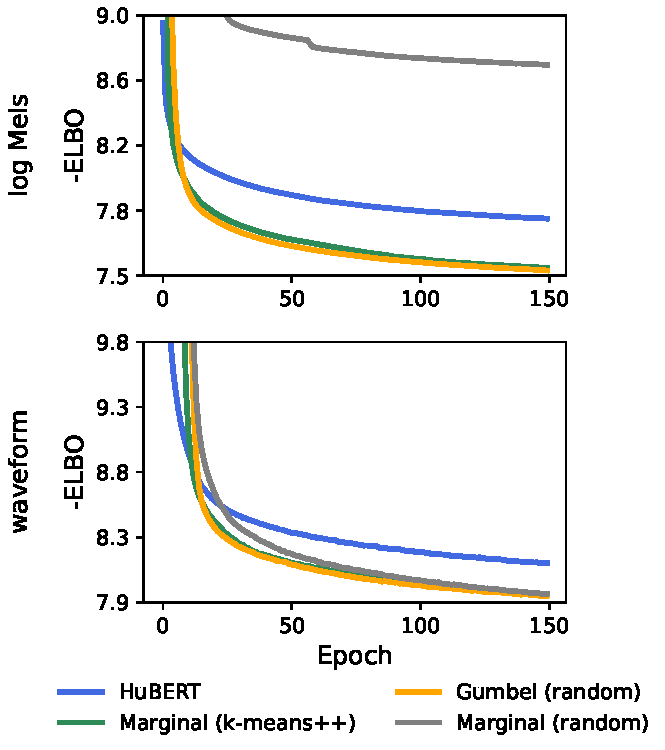
\includegraphics[width=7cm]{plots/plot_optimization.pdf}
    \caption{The training losses of different optimization approaches
      implemented by our own \textsc{Base} (top) and in fairseq \textsc{Base} (bottom).
      The final loss values can be found in Table~\ref{tab:ctc}.}
    \label{fig:optimization}
\end{figure}


%
%
%
%
%
%
%
%
%
%
%
%
%
%
%
%
%
%
%
%
%
%
%
%
%
%
%
%
%
%
%
%
%
%
%
%
%
%
%
%
%
%
%
%
%
%
%
%
%
%
%
%
%
%
%


%
%
%
%
%
%
%
%
%
%
%
%
%
%
%
%
%
%
%
%
%
%
%
%
%
%
%
%
%
%
%
%
%
%
%
%
%
%
%
%
%
%
%
%
%
%
%
%
%
%
%
%
%
%
%
%
%
%
%
%
%
%
%
%
%
%
%
%
%
%
%
%
%
%
%
%
%
%
%
%
%
%

\subsection{Downstream Evaluation}

Given that we can improve pre-training, the next question is whether the improvement transfer to downstream tasks.
Besides, our framework allows for controlled experiments that only differ in loss functions while holding everything else, such as the model architecture and training hyperparameters, fixed.
Based on the connections to prior work in Section \ref{sec:related}, we will study two important design choices, i.e., comparing masked prediction to future prediction and comparing the contrastive loss in wav2vec 2.0 to the softmax in the HuBERT objective.

The utility of speech representations on downstream tasks are evaluated with probing \citep{oord2018representation, chung2019unsupervised, yang2022autoregressive, yang21c_interspeech}, where the pre-trained models are frozen and small classifiers are trained to complete tasks given the hidden vectors of one of the layers.

%
%
%
%
%
%
%
%

We conduct four probing tasks, phone classification, speaker verification, fundamental frequency tracking, and automatic speech recognition.
All settings follow \citet{yang2022autoregressive} unless otherwise noted.
For phone classification, we train a linear classifier to predict phone labels obtained from forced alignments on the Wall Street Journal \citep{paul1992design} (WSJ).
We report phone error rates (PERs) on \texttt{dev93} and \texttt{eval92}, using 
10\% of the training set \texttt{si284} for development.
For f0 tracking, we train a linear regression model to predict the f0 extracted with PYIN \citep{mauch2014pyin} on WSJ.
We report the root-mean-square error (RMSE) in Hz on \texttt{eval92}.
For speaker verification, we train a two-layer classifier to predict speaker identities on VoxCeleb1 \citep{nagrani2020voxceleb} and use the intermediate layer as the speaker embedding for speaker verification.
We report equal error rates (EERs) on the test set.
The reported numbers are with the best layer for each task and for each model.
More details are in Appendix \ref{appendix:downstream}.

%
%
%
%
%
%
%
%
%
%
%
%

%
%
%
%
%
%
%

%
%
%
%
%

\begin{table}
    \caption{Downstream probing results for different speech representations
        on phone classification, speaker verification, and f0 tracking.}
    \label{tab:downstream1}
    \centering
    %
    \footnotesize
    \begin{tabularx}{0.98\linewidth}{lcccc}
    %
            \toprule
             %
                    &\multicolumn{2}{c}{PER $\downarrow$} &EER $\downarrow$ &RMSE $\downarrow$  \\
                    &dev93 &eval92 &voxceleb &eval92  \\[1pt]
            \midrule
            %
            log Mel       &49.8          &50.0       &24.6        &38.4 \\
            i-vector      &-             &-          &15.7        &-    \\
            %
            %
            %
            %
            %
            %
            %
            %
            %
            HuBERT Obj            &12.8          &12.6          &18.3      &23.4  \\
            Masked-VPC        &11.8          &11.3          &14.4      &20.9  \\
            %
            \bottomrule
    %
    \end{tabularx}
    %
\end{table}

\paragraph{Better pre-training leads to better downstream performance}

We have shown that using soft assignment and sampling gives us the best pre-training loss.
To answer whether the improved pre-training transfer to downstream tasks,
we compare HuBERT Obj with the soft assignment variant optimized with sampling and Gumbel softmax (termed Masked-VPC).
Results on three tasks are shown in Table \ref{tab:downstream1}.
We see that improving pre-training indeed improves downstream tasks across the board.
ASR results are deferred to later sections, but the conclusion stands.

%
%
%
%
%
%
%
%
%

\begin{table}
    \caption{Downstream probing results comparing future prediction (Future-VPC) and masked prediction (Masked-VPC) on phone classification, speaker verification, and f0 tracking.}
    \label{tab:downstream2}
    \centering
    \footnotesize
    \begin{tabularx}{0.98\linewidth}{lcccc}
        \toprule
           &\multicolumn{2}{c}{PER $\downarrow$} &EER $\downarrow$ &RMSE $\downarrow$  \\
           &dev93 &eval92 &voxceleb &eval92  \\[1pt]
        \midrule                                                                                                                 
        %
        %
        %
        %
        %
        %
        %
        Masked-VPC          &11.8          &11.3           &14.4     &20.9  \\
        Future-VPC          &16.0          &15.5           &13.6     &20.5  \\
        \bottomrule
    \end{tabularx}
\end{table}

\paragraph{Future prediction can be as strong as masked prediction on some downstream tasks}

As shown in Section \ref{sec:futurepred}, under our framework, it is possible (and relatively simple) to switch from masked prediction to future prediction while holding everything else fixed.
Future prediction is more relevant than masked prediction in certain scenarios, such as streaming or pre-training decoder-only Transformers.
\citet{misra21_interspeech}, for example, show that future prediction can be as strong as masked prediction for streaming ASR.
Results comparing future prediction (Future-VPC) and masked prediction (Masked-VPC) are shown in Table \ref{tab:downstream2}.
We find that, not surprisingly, future prediction is worse at phone classification compared to masked prediction.
However, future prediction is better than masked prediction on speaker verification and fundamental frequency tracking.

%
%
%
%
%
%
%

\begin{table}
    \caption{Downstream probing results comparing NCE (Masked-NCE), i.e., using a contrastive loss with the HuBERT approaches (HuBERT Obj and Masked-VPC) on phone classification, speaker verification, and f0 tracking.}
    \label{tab:downstream3}
    \centering
    %
    \footnotesize
    \begin{tabularx}{0.98\linewidth}{lcccc}
    \toprule
       &\multicolumn{2}{c}{PER $\downarrow$} &EER $\downarrow$ &RMSE $\downarrow$  \\
       &dev93 &eval92 &voxceleb &eval92  \\[1pt]
    \midrule                                                                                                                 
    %
    Masked-NCE       &12.2          &12.4      &20.2        &24.4       \\
    HuBERT Obj           &12.8          &12.6      &18.3        &23.4       \\
    Masked-VPC       &11.8          &11.3      &14.4        &20.9       \\
    \bottomrule
    \end{tabularx}
\end{table}

\paragraph{NCE is on par with HuBERT Obj}

%
%
%
%
%

To compare to the contrastive loss, we parameterize $q(z_i|x_i)$ and $p(z_i | x_{\setminus M})$ as detailed in Section \ref{sec:wav2vec}. 
We characterize the model in Table \ref{tab:model-summary} and denote it as Masked-NCE.
The entropy term is a constant because of the Dirac delta.
%
We follow \citet{baevski2020wav2vec} and take the negative samples for NCE from frames within the same batch.
The codebook is updated together with the contrastive loss with Gumbel softmax as in \citet{baevski2020wav2vec}.
Results are shown in Table \ref{tab:downstream3}.
NCE alone performs surprisingly well and closely matches HuBERT's results, while our approach is still superior.
%

%
%
%
%
%
%
%
%


%
%
%

%
%
%
%
%
%
%
%
%
%
%

%
%
%
%
%
%
%
%

%
%
%
%

%
%
%
%


%
%
%
%
%
%
%
%
%
%
%
%
%
%
%
%
%
%
%
%
%
%
%
%
%
%
%
%
%
%

\begin{table}[t]
  \caption{Probing results with lexicon-free seq2seq models on WSJ.
    No language models are used.}
  \label{tab:downstream_asr}
  \centering
  \begin{threeparttable}
  \footnotesize
  \addtolength{\tabcolsep}{-0.11em}
  \begin{tabularx}{0.94\linewidth}{lcccc}
    \toprule
      &\multicolumn{2}{c}{CER $\downarrow$} &\multicolumn{2}{c}{WER $\downarrow$}\\
            &dev93 &eval92  &dev93 &eval92\\[1pt]
    \midrule
    \multicolumn{4}{l}{\textbf{\textsc{Baseline}}}  \\[2pt]
    wav2letter++ \tnote{\dag}   &6.3   &4.1    &19.5     &13.9\\
    18L Transformer\tnote{\ddag}&- &- &22.2     &17.9\\
    \midrule                                                                                                                 
    \multicolumn{4}{l}{\textbf{\textsc{Probing with our seq2seq}}}  \\[2pt]
    log Mel     &6.8   &5.1  &18.2      &14.7 \\
    VQ-APC      &5.8  &5.2    &16.8      &14.9  \\
    Future-VPC   &5.4  &4.0    &15.5      &12.4  \\
    Masked-NCE   &5.0  &4.9    &14.5      &14.4  \\
    HuBERT Obj     &5.2  &5.0    &15.2      &14.5  \\
    Masked-VPC   &4.4  &3.6    &13.6      &11.4  \\
    \bottomrule
  \end{tabularx}
  \begin{tablenotes}\footnotesize
  \item[\dag] Numbers taken from \citet{baevski2019vq}.
  \item[\ddag] Numbers taken from \citet{higuchi2020mask}. 
  \end{tablenotes}
  \end{threeparttable}
\end{table}

\subsection{Automatic Speech Recognition}

Automatic speech recognition (ASR) has been the main driving force behind speech representation 
learning. In this section, we evaluate the quality of speech representations with two ASR settings, a probing setting with sequence-to-sequence (seq2seq) models and a fine-tuning setting with connectionist temporal classification (CTC).
We report CERs and WERs averaged over three runs. 

\paragraph{Probing with seq2seq}

In the probing setting, we follow \citet{yang2022autoregressive}, extracting the layer that achieves the best phone classification, and train a seq2seq model with character outputs on WSJ.\footnote{
More training details are in Appendix \ref{appendix:downstream}.}
Following the spirit of probing, we make sure that the improvement is solely from the learned representations 
and that the phonetic information is accessible, by not using a language model or a lexicon,
and by using a lightweight model.
Beam search is used with a beam size of~5.

Table~\ref{tab:downstream_asr} reports the ASR performance in terms of character error rates (CERs) and word error rates (WERs).
Despite being lightweight, our baseline model on log Mel features is by no means weak, and is on par with wav2letter++ in \citet{8683535} and 
better than a 18-layer Transformer baseline in \citet{higuchi2020mask}.
We then compare representations learned from the approaches characterized in Table \ref{tab:model-summary}, including two future prediction approaches (VQ-APC, Future-VPC) and three masked prediction approaches (Masked-NCE, HuBERT Obj, Masked-VPC).
We first find that representations learned from future prediction are not far behind those from masked prediction.
The second is that the improvement from HuBERT Obj to Masked-VPC (in Section \ref{sec:opt}) transfers well to ASR as well.

\begin{table}[t]
\centering
\captionof{table}{Results of ASR fine-tuned on WSJ using CTC
  for different optimization approaches during pre-training.
  No language models are used.
}
\label{tab:ctc}
\begin{threeparttable}
\footnotesize
\begin{tabularx}{0.94\linewidth}{lcccc}
  \toprule
     &$-$ELBO &dev93 &eval92\\[1pt]
  \midrule
  \multicolumn{3}{l}{\textbf{\textsc{Fine-Tuning (Ours)}}} &\\[1pt]
  HuBERT Obj               &7.79 &15.5 &12.5  \\
  Marginal ($k$-means++)     &7.50 &14.3 &11.0  \\
  Marginal (random)        &8.70 &15.0 &11.7  \\
  Gumbel (random)          &7.48 &14.1 &11.7  \\
  \midrule
  \multicolumn{3}{l}{\textbf{\textsc{Fine-Tuning (Fairseq)}}} &\\[1pt]
  HuBERT Obj               &8.14 &14.9 &11.8  \\
  Marginal ($k$-means++)     &7.91 &14.5 &11.1  \\
  Marginal (random)        &7.91 &14.2 &10.9  \\
  Gumbel (random)          &7.89 &14.3 &11.0  \\
  \bottomrule
\end{tabularx}
\end{threeparttable}
\end{table}


\paragraph{Fine-tuning with CTC}

%
%
To further confirm that improvement in pre-training transfers to ASR,
we fine-tune the pre-trained models on WSJ \citep{paul1992design} using CTC \citep{graves2006connectionist} with characters output. 
%
%
We fine-tune our \textsc{Base} for 100 epochs and fairseq \textsc{Base} for 200 epochs on \texttt{si284}.
%
%
%
Similar to \citet{lee2021intermediate,higuchi2020mask},
we average models from last 10 epochs after training to obtain final model parameters.
%
Table \ref{tab:ctc} summarizes the pre-training losses (-ELBO) reported in Figure~\ref{fig:optimization} and 
the corresponding WERs on \texttt{dev93} and \texttt{eval92}. The inference is done with greedy decoding.
%
%
%
The improvement in objective indeed transfers well to ASR in both settings.

To see whether the improvement is still present when decoding with a language model, Table~\ref{tab:ctc-lm} compared the results after using a 4-gram word language model \citep{heafield2013scalable}.
A beam size of 2000 is used for decoding with the 4-gram language model.
The improvement transfer well even with the use of a language model.

Lastly, to see the effect on small datasets, we follow \citet{baevski2020wav2vec} and evaluate phonetic recognition on TIMIT.
%
%
%
%
%
%
We observe the same trend in Table \ref{tab:ctc2} that our approach consistently performs better than HuBERT Obj.

\begin{table}[t]
\centering
\captionof{table}{Comparing ASR fine-tuned on WSJ using CTC with and without a 4-gram language model.
}
\label{tab:ctc-lm}
\begin{threeparttable}
\footnotesize
\begin{tabularx}{0.97\linewidth}{lccccc}
  \toprule
                                & \multicolumn{2}{c}{w/o LM} &\multicolumn{2}{c}{w/ LM} \\
                                & dev93 & eval92  &dev93 &eval92 \\
  \midrule
  \textbf{\textsc{Baseline}} &&&&\\[1pt]
    12L Transformer\tnote{\ddag} &20.1 &16.5 &- &-\\
    wav2letter++ \tnote{\dag}     &19.5     &8.57 &&\\
  %
  \midrule
  \multicolumn{3}{l}{\textbf{\textsc{Fine-Tuning}}} &\\[1pt]
  %
  %
    Masked-NCE                     &14.7 &11.1  &7.8 &4.4 \\
    HuBERT Obj                     &15.5  &12.5 &7.3  &4.6\\
    Masked-VPC                     &14.1  &10.3 &6.8  &4.6\\
  \bottomrule
\end{tabularx}
\begin{tablenotes}\footnotesize
\item[\ddag] Numbers taken from \citet{lee2021intermediate}.
\item[\dag] Numbers taken from \citet{baevski2019vq}.
\end{tablenotes}
\end{threeparttable}
\end{table}

\begin{table}[t]
  \centering
  \caption{Phone recognition fine-tuned with CTC on TIMIT.}
  \label{tab:ctc2}
  \footnotesize
  \begin{tabular}{lccc}
    \toprule
                             &dev PER     &test PER $\downarrow$ \\
    \midrule
    \textbf{\textsc{Baseline}} &\\[1pt]
    12L Transformer &22.1 &24.1\\
    \midrule
    \multicolumn{2}{l}{\textbf{\textsc{Fine-Tuning}}} \\[1pt]
    %
    %
    Masked-NCE      &11.2  &12.9 \\
    HuBERT Obj      &10.2  &11.3 \\
    Masked-VPC      &9.5   &11.0 \\
    \bottomrule
  \end{tabular}
\end{table}

\subsection{Second-Iteration Training}

As detailed in Section \ref{sec:hubert-variants},
our framework can be extended to the second iteration
as in HuBERT \citep{hsu2021hubert}.
%
%
%
%
%
%
%
%
%
%
%
%
%
Following \citet{hsu2021hubert}, the Transformer encoder
from the previous iteration is held fixed in the second iteration.

We run the second iteration using fairseq, based on the its first iteration in Figure \ref{fig:optimization} (bottom). 
For the proposed approach, we choose Masked-VPC with $k$-means++ initialization from the first iteration, 
applying the same initialization to the second iteration training.
We adopt the 6-th layer of Transformers of HuBERT and Masked-VPC in the previous iteration, the layer that provides the best downstream ASR performance in Table \ref{tab:downstream_asr}.
We use a temperature $\tau$ of 10 to avoid $q$ being one-hot.
We train second-iteration HuBERT and Masked-VPC for 150 epochs, and evaluate them with CTC finetuning 
as in the previous section.

As shown in Table~\ref{tab:ctc-iter2}, the second iteration improves both approaches by a large margin.
In particular, we observe 4.1\% reduction of WER on \texttt{dev93} with our approach. 
Moreover, the improvements in objective transfers to the second iteration, in which 
Masked-VPC obtains 0.7\% and 0.3\% lower WERs than HuBERT on each set.
Similar trend is observed with an ngram language model for CTC decoding.


\begin{table}[t]
\centering
\captionof{table}{Second-iteration results of ASR fine-tuned on WSJ using CTC with or without an ngram LM.}
\label{tab:ctc-iter2}
\footnotesize
\begin{tabular}{lccccc}
  \toprule
  & \multicolumn{2}{c}{w/o LM} & \multicolumn{2}{c}{w/ LM}\\
  &dev93 &eval92 &dev93 &eval92\\[1pt]
  \midrule
  \multicolumn{3}{l}{\textbf{\textsc{First iteration}}} &\\[1pt]
  HuBERT Obj                  &14.9 &11.8 &7.9 &6.0\\
  Masked-VPC                &14.5 &11.1 &7.8 &5.3 \\
  \midrule
  \multicolumn{3}{l}{\textbf{\textsc{Second iteration}}} &\\[1pt]
  HuBERT Obj                &11.1 &8.2  &6.2 &4.2 \\
  Masked-VPC                &10.4 &7.9  &5.9 &3.8 \\
  \bottomrule
\end{tabular}
\end{table}
